\documentclass[3p,10pt]{elsarticle}
\usepackage{latexsym,epsf,amssymb,amsthm,amsfonts,multicol,makeidx}
\usepackage{color}
\usepackage{colortbl,xcolor}
\usepackage{epsfig,amssymb}
\usepackage{amsmath}
\usepackage{tikz}
\usepackage{pgfplots}
\usetikzlibrary{arrows}
\usetikzlibrary[patterns]

\begin{document}

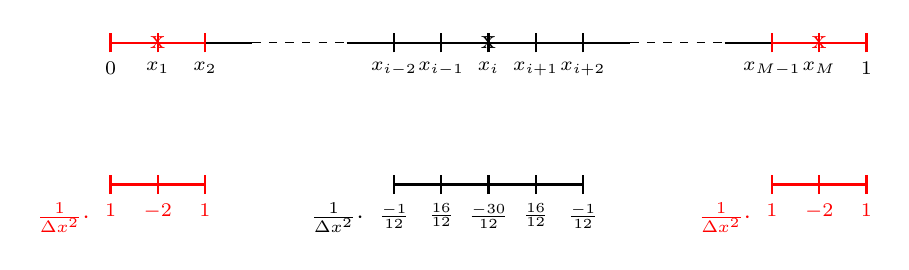
\begin{tikzpicture}[x=1cm,y=1cm,scale=0.6]

\draw[thick,red] (0,0)--(2,0);
\draw[thick] (2,0)--(3,0);
\draw[dashed] (3,0)--(5,0);
\draw[thick] (5,0)--(11,0);
\draw[dashed] (11,0)--(13,0);
\draw[thick] (13,0)--(14,0);
\draw[thick,red] (14,0)--(16,0);

\draw[thick,red] (0,-0.2)--(0,0.2);
\draw[thick,red] (1,-0.2)--(1,0.2);
\draw[thick,red] (2,-0.2)--(2,0.2);
\draw[thick] (6,-0.2)--(6,0.2);
\draw[thick] (7,-0.2)--(7,0.2);
\draw[thick] (8,-0.2)--(8,0.2);
\draw[thick] (9,-0.2)--(9,0.2);
\draw[thick] (10,-0.2)--(10,0.2);
\draw[thick,red] (14,-0.2)--(14,0.2);
\draw[thick,red] (15,-0.2)--(15,0.2);
\draw[thick,red] (16,-0.2)--(16,0.2);
\draw[thick,red] (1,0) node[]  {\normalsize x};
\draw[thick] (8,0) node[]  {\normalsize x};
\draw[thick,red] (15,0) node[]  {\normalsize x};
%
%
\draw [] (0,-0.2) node[below]  {\scriptsize $0$};
\draw [] (1,-0.2) node[below]  {\scriptsize $x_1$};
\draw [] (2,-0.2) node[below]  {\scriptsize $x_2$};
\draw [] (6,-0.2) node[below]  {\scriptsize $x_{i-2}$};
\draw [] (7,-0.2) node[below]  {\scriptsize $x_{i-1}$};
\draw [] (8,-0.2) node[below]  {\scriptsize $x_i$};
\draw [] (9,-0.2) node[below]  {\scriptsize $x_{i+1}$};
\draw [] (10,-0.2) node[below]  {\scriptsize $x_{i+2}$};
\draw [] (14,-0.2) node[below]  {\scriptsize $x_{M-1}$};
\draw [] (15,-0.2) node[below]  {\scriptsize $x_M$};
\draw [] (16,-0.2) node[below]  {\scriptsize $1$};


\draw[thick,red] (0,-3)--(2,-3);
\draw[thick,red] (0,-3.2)--(0,-2.8);
\draw[thick,red] (1,-3.2)--(1,-2.8);
\draw[thick,red] (2,-3.2)--(2,-2.8);

\draw [red] (-1,-3.7) node[]  {\small $\frac{1}{\Delta x^2} \cdot $};

\draw [red] (0,-3.2) node[below]  {\scriptsize $1$};
\draw [red] (1,-3.2) node[below]  {\scriptsize $-2$};
\draw [red] (2,-3.2) node[below]  {\scriptsize $1$};


\draw[thick] (6,-3)--(10,-3);

\draw[thick] (6,-3.2)--(6,-2.8);
\draw[thick] (7,-3.2)--(7,-2.8);
\draw[thick] (8,-3.2)--(8,-2.8);
\draw[thick] (9,-3.2)--(9,-2.8);
\draw[thick] (10,-3.2)--(10,-2.8);

\draw [] (4.8,-3.7) node[]  {\small $\frac{1}{\Delta x^2} \cdot $};

\draw [] (6,-3.2) node[below]  {\scriptsize $\frac{-1}{12}$};
\draw [] (7,-3.2) node[below]  {\scriptsize $\frac{16}{12}$};
\draw [] (8,-3.2) node[below]  {\scriptsize $\frac{-30}{12}$};
\draw [] (9,-3.2) node[below]  {\scriptsize $\frac{16}{12}$};
\draw [] (10,-3.2) node[below]  {\scriptsize $\frac{-1}{12}$};


\draw[thick,red] (14,-3)--(16,-3);
\draw[thick,red] (14,-3.2)--(14,-2.8);
\draw[thick,red] (15,-3.2)--(15,-2.8);
\draw[thick,red] (16,-3.2)--(16,-2.8);

\draw [red] (13,-3.7) node[]  {\small $\frac{1}{\Delta x^2} \cdot $};

\draw [red] (14,-3.2) node[below]  {\scriptsize $1$};
\draw [red] (15,-3.2) node[below]  {\scriptsize $-2$};
\draw [red] (16,-3.2) node[below]  {\scriptsize $1$};

\end{tikzpicture}

\end{document}